\section{Operationsverstärker}
\subsection{Opamp Schaltungen (allgemein gilt: $V_{out} = A_{ol}[(V_+ + V_{OS})-V_-]$)}
	\subsubsection{Invertierender Verstärker}
    \begin{minipage}[T]{13cm}
      Closed-Loop Verst\"arkung
      \hspace{3mm}\fbox{$V_{out} = \frac{-A_{ol}\cdot\frac{R_2}{R_1+R_2}}{1+A_{ol}\cdot \frac{R_1}{R_1+R_2}}\cdot V_{in} \cong -\frac{R_2}{R_1}      \cdot V_{in}$}\\
		  inkl. Offsetspannung
		  \hspace{10.2mm}\fbox{$V_{out} = \frac{A_{ol}}{1+A{ol}\cdot \frac{R_1}{R_1+R_2}}\cdot \left[(V_{AGND}+V_{OS})-V_{in} \cdot \frac{R_2}{R_1+R_2      }\right]$}\\
      f\"ur $A{ol}$ gross
      \hspace{22mm}\fbox{$V_{out} = \frac{R_1+R_2}{R_1}\cdot (V_{AGND}+V_{OS})-\frac{R_2}{R_1}\cdot V_{in}$}\\
      Ausgangswiderstand    \hspace{10.5mm}\fbox{$r_{out}=0\Omega$}\\
      Eingangswiderstand    \hspace{11mm}\fbox{$r_{in}=R_1$}
    \end{minipage}
		\begin{minipage}{6cm}
      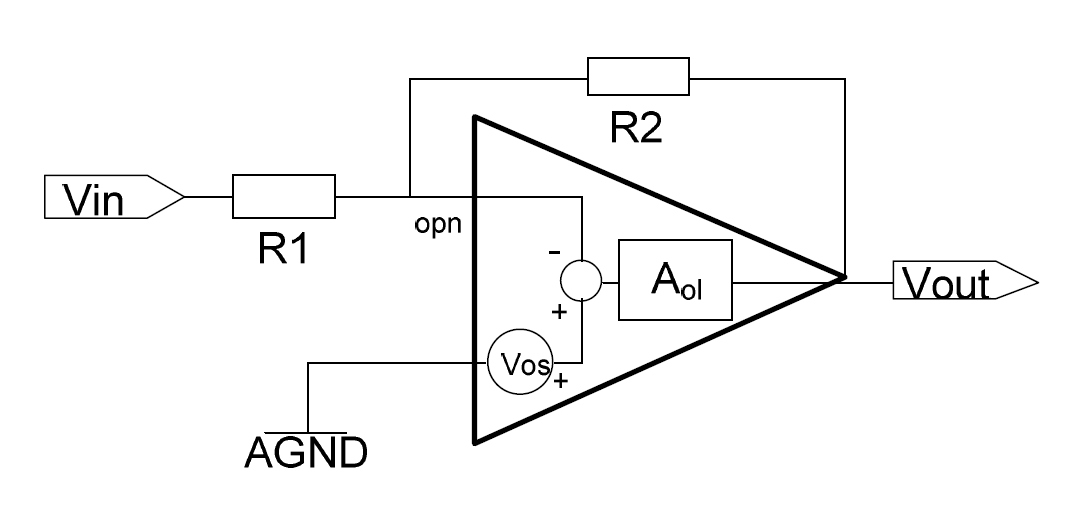
\includegraphics[width=6cm]{./bilder/i-verstaerker.png}
    \end{minipage}\\
\hrule

	\subsubsection{Nichtinvertierender Verstärker}
		\begin{minipage}[T]{13cm}
      Closed-Loop Verst\"arkung
      \hspace{3mm}\fbox{$V_{out} = \frac{A_{ol}}{1+A_{ol}\cdot \frac{R_1}{R_1+R_2}} \cdot V_{in} \cong \left( 1+\frac{R_2}{R_1}\right)  \cdot V_{      in}$}\\
      inkl. Offsetspannung
      \hspace{10.2mm}\fbox{$V_{out} = \frac{A_{ol}}{1+A_{ol}\cdot\frac{R_1}{R_1+R_2}}\cdot(V_{in}+V_{OS})$}\\
      f\"ur $A{ol}$ gross
      \hspace{22mm}\fbox{$V_{out} =\left(1 + \frac{R_2}{R_1}\right) \cdot (V_{in}+V_{OS})$}\\
      Ausgangswiderstand    \hspace{10.5mm}\fbox{$r_{out}=0\Omega$}\\
      Eingangswiderstand    \hspace{11mm}\fbox{$r_{in}=\infty$}\\
    \end{minipage}
		\begin{minipage}{6cm}
      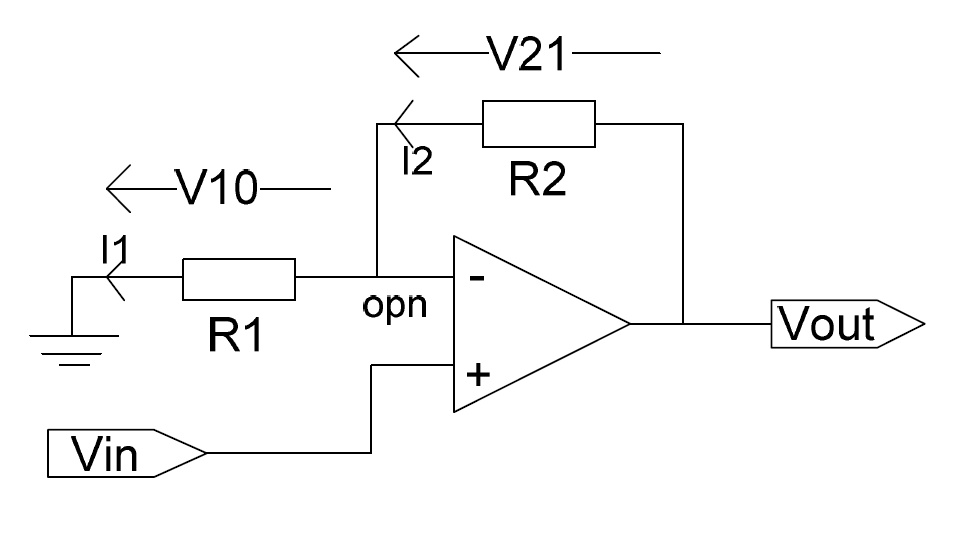
\includegraphics[width=6cm]{./bilder/ni-verstaerker.png}
    \end{minipage}\\
\hrule

  \subsubsection{Invertierender Addierer}
    \begin{minipage}[T]{13cm}
      Closed-Loop Verst\"arkung
      \hspace{3mm}\fbox{$V_{out}= -R_F \cdot \left(V_{in1}\cdot \frac{1}{R_1} + V_{in2}\cdot \frac{1}{R_2}+ \ldots\right) $}\\
      \hspace*{43mm}\fbox{$A_{CL1}=- \frac{R_F}{R_1}$}
      ;\hspace{0.2mm} \fbox{$A_{CL2}=- \frac{R_F}{R_2}$}
      ; \ldots
    \end{minipage}
    \begin{minipage}{6cm}
      \includegraphics[width=6cm]{./bilder/invertadd.png}
    \end{minipage}\\
  
  \hrule
	\subsubsection{Verstärker mit mehreren Eingängen}
		\begin{minipage}[T]{13cm}
      Closed-Loop Verst\"arkung
      \hspace{3mm}\fbox{$V_{out}=-\frac{R_F}{R_1}\cdot V_{in1}-\frac{R_F}{R_2}\cdot V_{in2}+\frac{R_F+(R_1//R_2)}{(R_1//R_2)}\cdot V_{in3}$}\\
      \hspace*{43mm}\fbox{$A_{CL1}=-\frac{R_F}{R_1}$}
      ;\hspace{0.3mm}\fbox{$A_{CL2}=-\frac{R_F}{R_2}$}
      ;\hspace{0.3mm}\fbox{$A_{CL3}=\frac{R_F+(R_1//R_2)}{(R_1//R_2)}$}\\
    \end{minipage}
		\begin{minipage}{6cm}
      \includegraphics[width=6cm]{./bilder/3-eingaenge.png}
    \end{minipage}\\
\hrule

	\subsubsection{Mehrfach-Addierer-Subtrahierer} 		
    \begin{minipage}[T]{13cm}
      1. Man w\"ahlt $R_{F}$\\
      2. Man w\"ahlt $R_{P}$, wobei oft $R_{P}=R_{F}$ gesetzt wird. (optional)\\
      3. $R_{n}=\frac{R_{F}}{\left|A_{n}\right|}$ oder
      $R_{n}=\frac{R_{P}}{\left|A_{n}\right|}$\\ 
      4. Verst\"rkungsbedingung: $A_{N1} +
      \ldots + A_{Nn} = A_{P1} + \ldots + A_{Pn}$ \\Falls unerf\"ullt, muss ein Dummyeingang hinzugefügt werden!
    \end{minipage}
    \begin{minipage}{6cm}
      \includegraphics[width=5.5cm]{./bilder/mehrfach-addierer-subtrahierer.png} 
    \end{minipage}\\
    
 \hrule
  

  \hrule        
	\subsubsection{Gewichteter Subtrahierer}
		\begin{minipage}[T]{13cm}
      Closed-Loop Verst\"arkung
      \hspace{3mm}\fbox{$V_{out}=\frac{R_3}{R_2+R_3}\left(1+\frac{R_F}{R_1}\right)\cdot V_{in2}-\frac{R_F}{R_1}\cdot V_{in1}$}\\
      f\"ur $R_3 = R_F$ und $R_2 = R_1$
      \hspace{0.1mm} \fbox{$V_{out}=\frac{R_F}{R_1}\cdot (V_{in2}-V_{in1})$}
    \end{minipage}
		\begin{minipage}{6cm}
      \includegraphics[width=6cm]{./bilder/gewichtsub.png}
    \end{minipage}\\		
\hrule

	\subsubsection{Differenzverstärker}
    \begin{minipage}[T]{14cm}
      Closed-Loop Verst\"arkung
      \hspace{3mm}\fbox{$V_{out} = \frac{R_3+R_4}{R_3}\cdot \left( \frac{R_1}{R_1+R_2}\cdot V_{ref} + \frac{R_2}{R_1+R_2}\cdot V_{in1}\right)-      \frac{R_4}{R_3}\cdot V_{in2} $}\\
      f\"ur $R_1 = R_3$ und $R_2 = R_4$
      \hspace{1mm} \fbox{$V_{out}= V_{ref} +\frac{R_4}{R_3}\cdot(V_{in1}-V_{in2})$}
    \end{minipage}
    \begin{minipage}{5cm}
      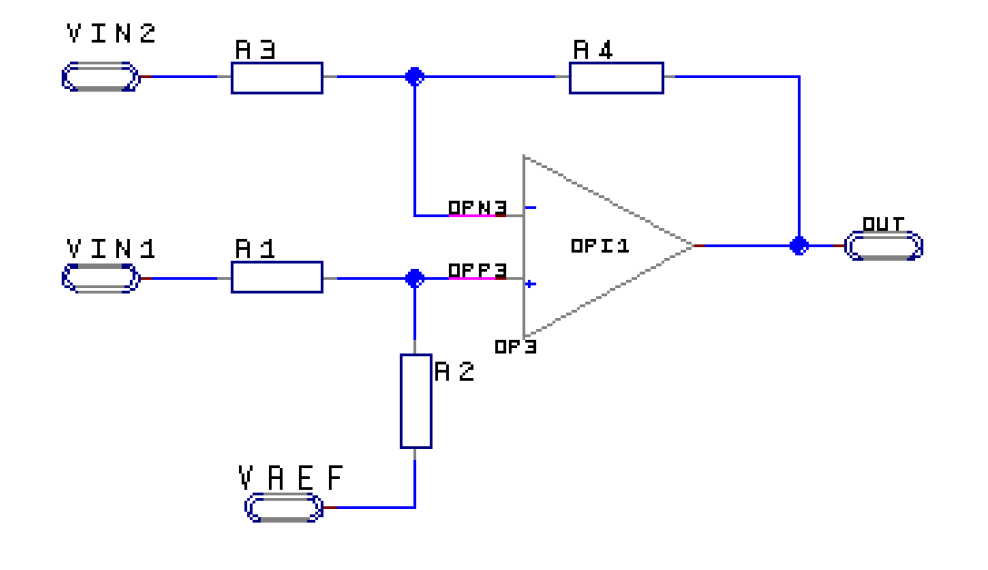
\includegraphics[width=5cm]{./bilder/differenzver.png}
    \end{minipage}\\
\hrule
        
	\subsubsection{Instrumentenverstärker}
		\begin{minipage}[T]{13cm}
      Stufe 1 (Pos Eingang)
      \hspace{18.8mm}\fbox{$V_{opo2} = V_{in2}+ \frac{R_{f2}}{R_G}\cdot(V_{in2}-V_{in1})$}\\
      Stufe 1 (Neg Eingang)
      \hspace{18.3mm}\fbox{$V_{opo1} = V_{in1}- \frac{R_{f1}}{R_G}\cdot(V_{in2}-V_{in1})$}\\
      Stufe 2 Closed-Loop Verst\"arkung
      \hspace{3.4mm}\fbox{$V_{out} = V_{ref}+\frac{R_4}{R_3}\cdot\left(1+\frac{R_{f1}+R_{f2}}{R_G} \right)\cdot (V_{in1}-V_{in2}) $}
		\end{minipage}
    \hspace{0.5cm}
		\begin{minipage}{6cm}
      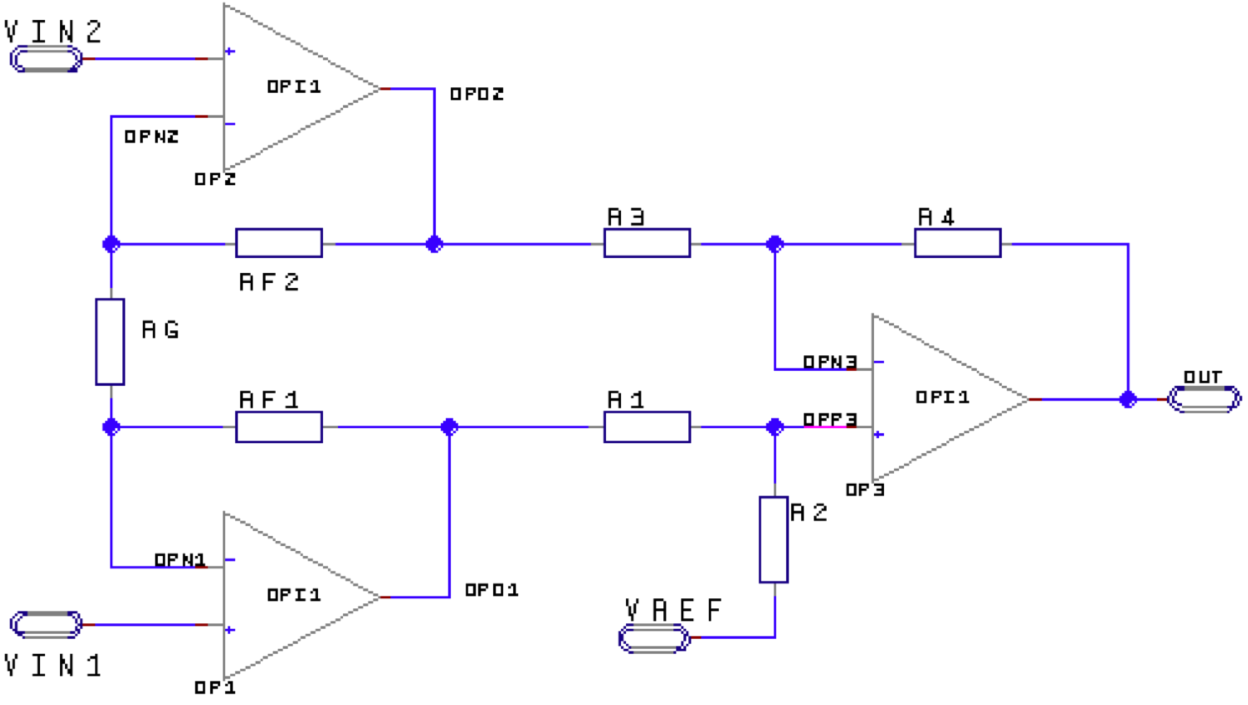
\includegraphics[width=6cm]{./bilder/Instrumentationsverstaerker.png} 
    \end{minipage}\\
  
  \hrule
  \subsubsection{T-Glied in Rückkopplung}
    \begin{minipage}[c]{12cm}
  	 	Für $A \to \infty$ (idealer OP) gilt: \smallskip \\
   	 	\fbox{$v_u=-\frac{R_2 \cdot R_3 + R_2 \cdot R_4 + R_3 \cdot R_4}{R_1 \cdot R_3}$}
   	 	\bigskip \\
   	 	$\Longrightarrow$ hohe Verstärkung mit kleinen Wertunterschieden - 
   	 	z.B.$R_1=R_3=1k\Omega$ und $R_2=R_4=10k\Omega$ ergibt $v_u=-120$ 
   	 	(Vergleich: $v_u=-10$ bei inv. Verstärker) \\
    \end{minipage}
    \hspace{0.5cm}
    \begin{minipage}[c]{5cm}
      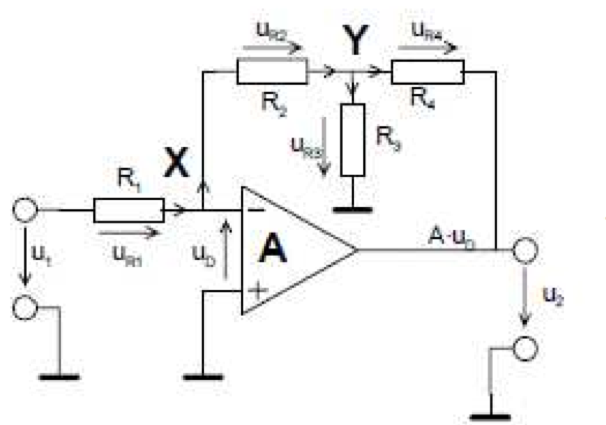
\includegraphics[width=5cm]{./bilder/tglied.png}
    \end{minipage}      

  \hrule 	 
  \subsubsection{Negative Impedance Converter (NIC)}
    \begin{minipage}[c]{12cm}    
      Der Negative Impedance Converter (NIC) stellt einen negativen reellen Widerstand
      dar. Verwendung: Kompensation parasitärer reeller Widerstände. \\
      Nachteil: Masse-Bezug des negativen Widerstands. \bigskip \\
      \fbox{$R_{EQ}=-R \cdot \frac{R_1}{R_2}$}\\
    \end{minipage}
    \begin{minipage}[c]{5cm}
      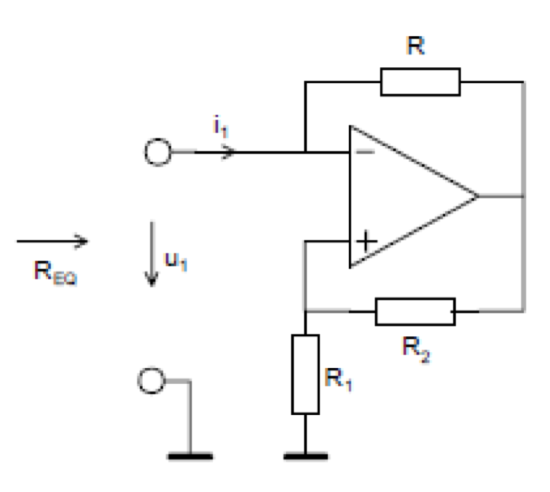
\includegraphics[width=5cm]{./bilder/neg-imp-conv.png}
    \end{minipage}


  \subsubsection{Integrator}
    \begin{minipage}[T]{13cm}
      Closed-Loop Verst\"arkung
      \hspace{3mm}\fbox{$V_{out} =-\frac{1}{R\cdot C} \int{V_{in}}dt + V_{out\hspace{1mm}Anfang}$}\\
      \hspace*{43mm}\fbox{$-\frac{1}{C} \int i_c dt + V_{out\hspace{1mm}Anfang}$}\\
      \hspace*{42mm} \fbox{$\frac{dv_{out}}{dt}=-\frac{v_{in}}{RC}$}\\ \\
      $R_F$ limitiert die Verst\"arkung bei tiefen Frequenzen. D.h. er wirkt als Tiefpass
    \end{minipage} 
    \begin{minipage}{6cm}
      \includegraphics[width=6cm]{./bilder/integrator.png} 
    \end{minipage}\\		
\hrule

  \subsubsection{Differentiator}
    \begin{minipage}[T]{13cm}
      Beim Differentiator gilt $V_{out}=v_N-i_1 \cdot R_F$ wobei $v_N=0$\\
      Closed-Loop Verst\"arkung
      \hspace{3mm}\fbox{$V_{out}=-R_F\cdot C_1 \frac{dv_{in}}{dt}$}\\
      \hspace*{43.2mm}\fbox{$i_1=C_1 \cdot \frac{dv_C}{dt}$}\\
      Die Elemente $C_F$ und $R_1$ sind optional. \\
      Sie beheben jedoch Probleme die ohne \\
      sie entstehen (siehe elemenarer Differentiator). \\
      Mit $C_F$ und $R_1$: \\
      - Keine differentiation bei h\"oheren Frequenzen. \\
      - Limitierte Verst\"arkung bei h\"oheren Frequenzen. \\
      - Eingangswiderstand immer gr\"osser $R_1$ $\rightarrow$ keine Belastung der Signalquelle\\
      - \textbf{Bandpass}-Charakteristik mit $\omega_1 = \frac{1}{R_1C_1}$; $\omega_2 = \frac{1}{R_FC_F}$
    \end{minipage}
    \begin{minipage}{6cm}
      \includegraphics[width=6cm]{./bilder/differentiator.png}
    \end{minipage}\\

  \hrule
  \subsubsection{Buffer (Spannungsfolger / Impedanzwandler)}
    \begin{minipage}[T]{13cm}
      Closed-Loop Verst\"arkung
      \hspace{3mm}\fbox{$V_{out} = \frac{A_{ol}}{1+A_{ol}}\cdot V_{in}\cong V_{in} $}\\
      inkl. Offsetspannung
      \hspace{10.2mm}\fbox{$V_{out} = \frac{A_{ol}}{1+A_{ol}}\cdot(V_{in}+V_{os})\cong V_{in}+V_{os}$}
    \end{minipage} 
    \begin{minipage}{6cm}
      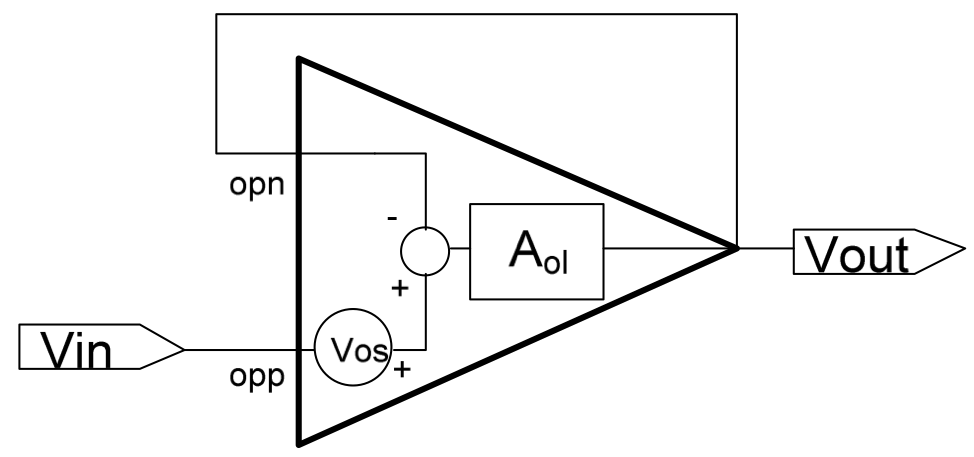
\includegraphics[width=6cm]{./bilder/buffer.png} 
    \end{minipage}\\		
\hrule

\subsection{Schmitt-Trigger}
  \subsubsection{Nicht invertierender Schmitt-Trigger}
		\begin{minipage}[T]{13cm}
      obere Schaltschwelle
      \hspace{10.8mm}\fbox{$V_{T+} = V_{ref}\cdot \frac{R_1+R_f}{R_f}-V_{out_{min}}\cdot\frac{R_1}{R_f}$}\\
      untere Schaltschwelle
      \hspace{9.6mm}\fbox{$V_{T-} = V_{ref}\cdot \frac{R_1+R_f}{R_f}-V_{out_{max}}\cdot\frac{R_1}{R_f}$}\\
      Hysteresespannung
      \hspace{12.8mm}\fbox{$V_{H} = V_{T+}-V_{T-} = (V_{out_{max}}-V_{out_{min}})\cdot\frac{R_1}{R_f}$}\\
    \end{minipage} 
    \begin{minipage}{6cm}
      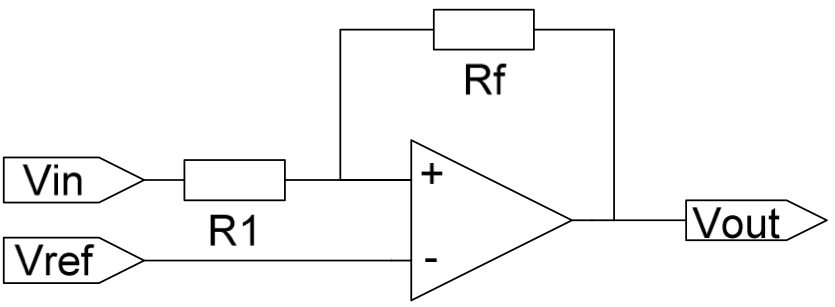
\includegraphics[width=6cm]{./bilder/n-schmitt.png} 
    \end{minipage}\\
            
  \subsubsection{Invertierender Schmitt-Trigger}
    \begin{minipage}[T]{13cm}
      obere Schaltschwelle
      \hspace{10.8mm}\fbox{$V_{T+} = \frac{V_{ref}\cdot R_f+ V_{out_{max}}\cdot R_1}{R_1+R_f}$}\\
      untere Schaltschwelle
      \hspace{9.6mm}\fbox{$V_{T-} = \frac{V_{ref}\cdot R_f+ V_{out_{min}}\cdot R_1}{R_1+R_f}$}\\
      Hysteresespannung
      \hspace{12.8mm}\fbox{$V_{H} = V_{T+}-V_{T-} = (V_{out_{max}}-V_{out_{min}})\cdot\frac{R_1}{R_1+R_f}$}\\ \\
      \textbf{Vorteil}: $V_{in}$ wird nicht unterschiedlich belastet!
    \end{minipage} 
    \begin{minipage}{6cm}
      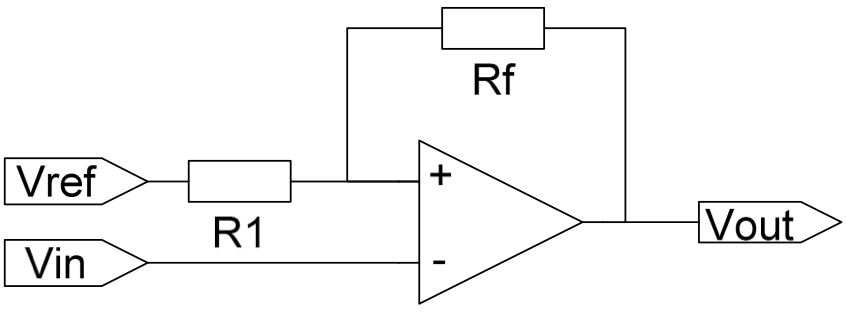
\includegraphics[width=6cm]{./bilder/i-schmitt.png} 
    \end{minipage}\\
            
  \subsubsection{Invertierender Schmitt-Trigger mit freien Schwellen}
    \begin{minipage}[T]{13cm}
      Schaltschwelle
      \hspace{20.8mm}\fbox{$V_{opp} =V_{ref}\cdot \frac{(R_f//R_0)}{R_1 +(R_f//R_0)}+V_{out}\cdot\frac{(R_1//R_0)}{R_f+(R_1//R_0)}$}\\ \\
      $V_{T+} \rightarrow V_{out} = V_{out_{max}} \qquad V_{T-} \rightarrow V_{out} = V_{out_{min}}$ \\
      Dimensionierung des Schmitt-Triggers: (Gegeben: $V_{ref}$, $V_{T+}$, $V_{T-}$)\\
      1. $V_{out_{max}}$ und $V_{out_{min}}$ ermitteln aus Datenblatt (meistens $V_{DD}$, $GND$)\\
      2. $R_f$ w\"ahlen: typisch $100 k\Omega$\\
      3. Widerst\"ande $R_1$ und $R_0$ dimensionieren\\
    \end{minipage} 
    \begin{minipage}{6cm}
      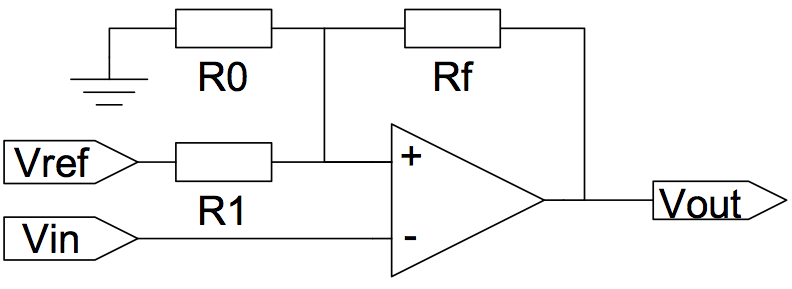
\includegraphics[width=6cm]{./bilder/i-schmittFreieSchwellen.png} 
    \end{minipage}\\
\hrule

\subsection{Gesteuerte Quellen}
  \begin{tabular}{|c|c|c|}
		\hline
		\multirow{2}{*}{Steuergrösse} & \multicolumn{2}{c|}{Ausgangsgrösse}\\ \cline{2-3}
		& V & I \\ \hline
		\multirow{8}{*}{V}	& Spannungsgesteuerte Spannungsquelle	& Spannungsgesteuerte Stromquelle		\\
    & \bf{VCVS} & \bf{VCCS} \\
		& Voltage Controlled Voltage Source		& Voltage Controlled Current Source \\ \cline{2-3}
		& 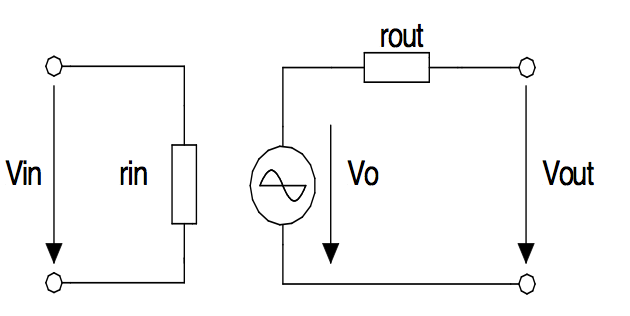
\includegraphics[width=4cm,trim=0 0 0 -5]{./bilder/vcvs.png}	
		& 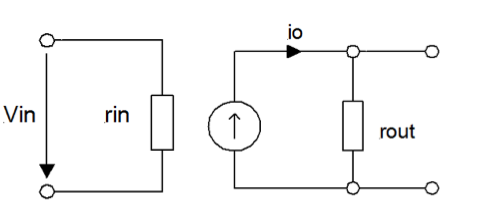
\includegraphics[width=4cm,trim=0 0 0 -5]{./bilder/vccs.png}  \\ \cline{2-3}
		& $v_{out}=v_{in} \cdot A_v$ & $i_{out} = v_{in} \cdot g_m$ \\
		& $A_v$: Spannungsverstärkung & $g_m$: Transkonduktanz  \\ \cline{2-3}
		& 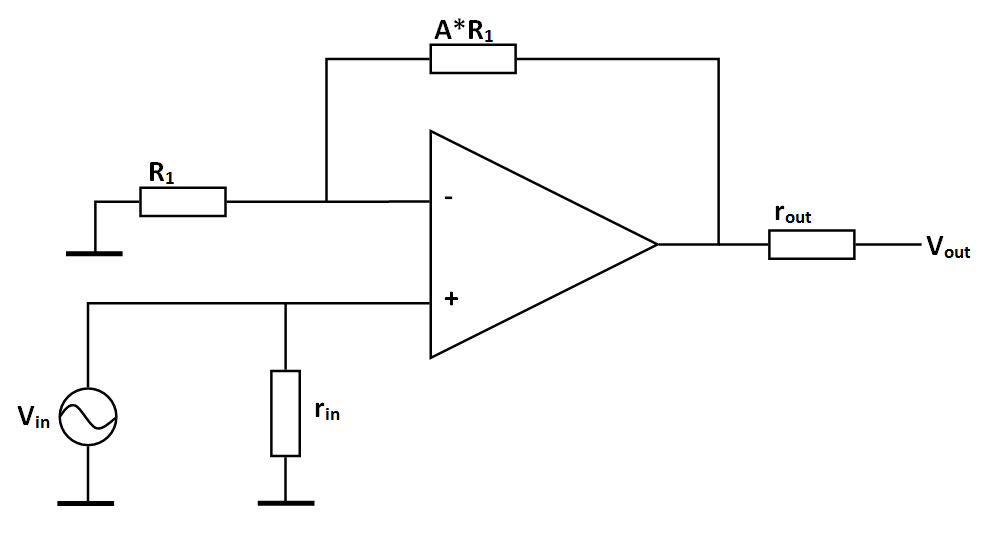
\includegraphics[width=4cm,trim=0 0 0 -5]{./bilder/vcvs_schaltung.png}
		& 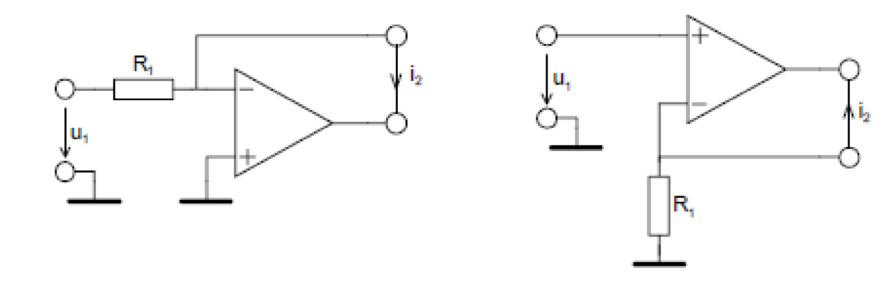
\includegraphics[width=4cm,trim=0 0 0 -5]{./bilder/vccs_schaltung.png}  \\
		&	& $I_2=\frac{V_1}{R_1}$ bzw. $I_2=-\frac{V_1}{R_1}$\\ 	\hline	
		\multirow{8}{*}{I}	& Stromgesteuerte Spannungsquelle		& Stromgesteuerte Stromquelle \\
		& \bf{CCVS} & \bf{CCCS} \\
		& Current Controlled Voltage Source	& Current Controlled Current Source \\ \cline{2-3}
		& 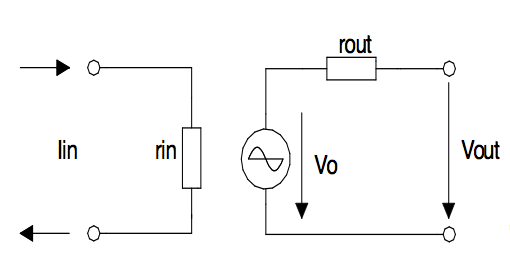
\includegraphics[width=4cm,trim=0 0 0 -5]{./bilder/ccvs.png}	
		& 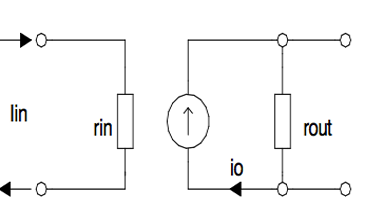
\includegraphics[width=4cm,trim=0 0 0 -5]{./bilder/cccs.png}  \\ \cline{2-3}
		& $v_{out}=i_{in} \cdot r_m$  & $i_{out} = i_{in \cdot A_i}$  \\
		& $r_m$: Transimpedanz  & $A_i$: Stromverstärkung \\ \cline{2-3}
		& 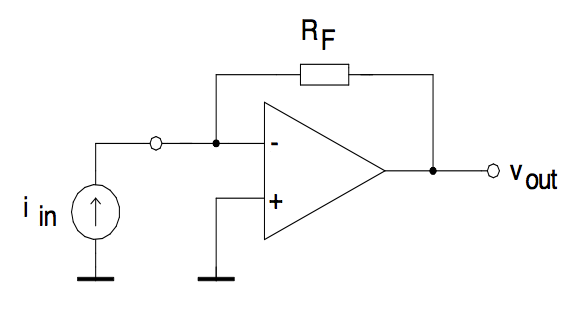
\includegraphics[width=4cm,trim=0 0 0 -5]{./bilder/tia.png}
		& 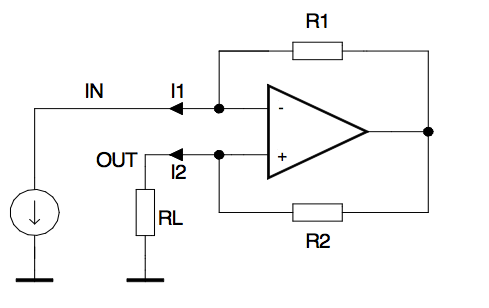
\includegraphics[width=4cm,trim=0 0 0 -5]{./bilder/cccs-schaltung.png}		\\ 
		& $v_{out}=-i_{in} \cdot r_F$ & $A_i=\frac{I_2}{I_1}=\frac{R_1}{R_2}$	\\ \hline
	\end{tabular} \\


\subsection{Nichtidealit\"aten des Operationsverst\"arkers}
  \subsubsection{Eingangsstromkompensation (Bias-Strom) ohne AC-Zweige (Kondensatoren)}
    \begin{minipage}[b]{6cm}
      \includegraphics[height=3cm]{./bilder/spannungsfolger.png}\\
      {\bf Spannungsfolger}\\ \\
      $R_2$ sei ein gegebener Quellenwiderstand\\
      $R_F$ muss eingefügt werden\\ \\
      \fbox{$R_F=R_2$}
    \end{minipage}\hfill
    \begin{minipage}[b]{6cm}
      \includegraphics[height=3cm]{./bilder/nichtinver}\\
      {\bf Nichtinvertierender Verstärker}\\ \\
      Hier sei der Quellenwiderstand vernachl\"assigbar.\\ 
      $R_2$ muss eingefügt werden\\ \\
      \fbox{$R_2=R_F//R_1$}
    \end{minipage}\hfill
    \begin{minipage}[b]{6cm}
    \includegraphics[height=3cm]{./bilder/inver}\\
      {\bf Invertierender Verstärker}\\ \\ \\ \\
      $R_2$ muss eingefügt werden\\ \\
      \fbox{$R_2=R_F//R_1$}
    \end{minipage}
    
    \begin{tabular}{p{7cm} l}
      \textbf{Ausgangsspannungsfehler} auf Grund des nicht 
      kompensierbaren \textbf{Offsetstroms} (nur bei Kompensation): &
      \begin{tabular}{l l}
        \fbox{$V_{out \hspace{1mm}E}=R_F\cdot (I_N-I_P) = R_F \cdot \left|I_{OS}\right|$}  &
        mit Eingangsstromkompensation \\
        \fbox{$V_{out \hspace{1mm}E}= R_F \cdot \left|I_N\right|$} &
        ohne Eingangsstromkompensation
      \end{tabular} \\
    \end{tabular}
    \begin{tabular}{l l l}
      \textbf{Bias Strom} & \fbox{$I_B = \frac{I_P + I_N}{2}$} & ist kompensierbar \\
      \textbf{Offset-Strom} & \fbox{$I_{OS}= \left| I_P - I_N \right|$} & nicht kompensierbar
    \end{tabular}
    

	\subsubsection{Zusammenfassung aller Fehlereinflüsse}
    \begin{minipage}[T]{12.5cm}
      \underline{{\bf Gleichtaktunterdr\"uckung} Common-Mode-Rejection Ratio $CMRR$}\\
            
      Offsetspannung
      \hspace{18.3mm}\fbox{$V_{OS}=\frac{V_{CM}}{CMRR_{lin}}$} mit \fbox{$V_{CM} = V_{opp} = V_{opn}$}\\
      Lineare Definition
      \hspace{14.2mm}\fbox{$CMRR_{lin}=\frac{dV_{CM}}{dV_{OS}}=10^{\frac{CMRR_{dB}}{20}}$}\\
      Logarithmische Definition
      \hspace{2.2mm}\fbox{$CMRR_{dB}=20 \cdot log(CMRR_{lin})=20 \cdot log\left( \frac{dV_{CM}}{dV_{OS}}\right) $}\\
      Ausgangs-Fehlerspannung
      \hspace{2.2mm}\fbox{$V_{out \hspace{1mm} E}=\left|V_{OS}\right| \cdot A_{CL+}=\left| \frac{\Delta V_{CM}}{CMRR_{lin}}\right|A_{CL+}$}
            
      \vspace{2mm}
      \underline{{\bf Power-Supply-Unterdrückungs-Fehler} Power-Supply-Rejection Ratio $PSRR$}\\
            
      Offsetspannung
      \hspace{18.3mm}\fbox{$V_{OS}=\frac{\Delta V_{Supply}}{PSRR_{lin}}$}\\
      Lineare Definition
      \hspace{14.2mm}\fbox{$PSRR_{lin}=\frac{dV_{Supply}}{dV_{OS}}=10^{\frac{PSRR_{dB}}{20}}$}\\
      Logarithmische Definition
      \hspace{2.2mm}\fbox{$PSRR_{dB}=20\cdot log(PSRR_{lin})=20\cdot log\left( \frac{dV_{Supply}}{dV_{OS}}\right) $}\\
      Ausgangs-Fehlerspannung
      \hspace{2.2mm}\fbox{$V_{out \hspace{1mm}E}=\left|V_{OS}\right| \cdot A_{CL+}=\left| \frac{\Delta V_{Supply}}{PSRR_{lin}}\right| A_{CL+}$}\\
            
      \vspace{2mm}
      \underline{\bf Gesamtfehlerspannung}\\
            
      \hspace*{43.3mm}\fbox{$V_{out\hspace{1mm}E\hspace{1mm}total}=A_{CL+}\cdot\left[\left|V_{OS}\right|+\frac{\left|V_{CM}\right|}{CMRR}+\frac{      \left|\Delta V_{Supply}\right|}{PSRR}\right]+\left|I_{OS}\right|\cdot R_F$}\\
    \end{minipage}
    \begin{minipage}[b]{6.5cm}
      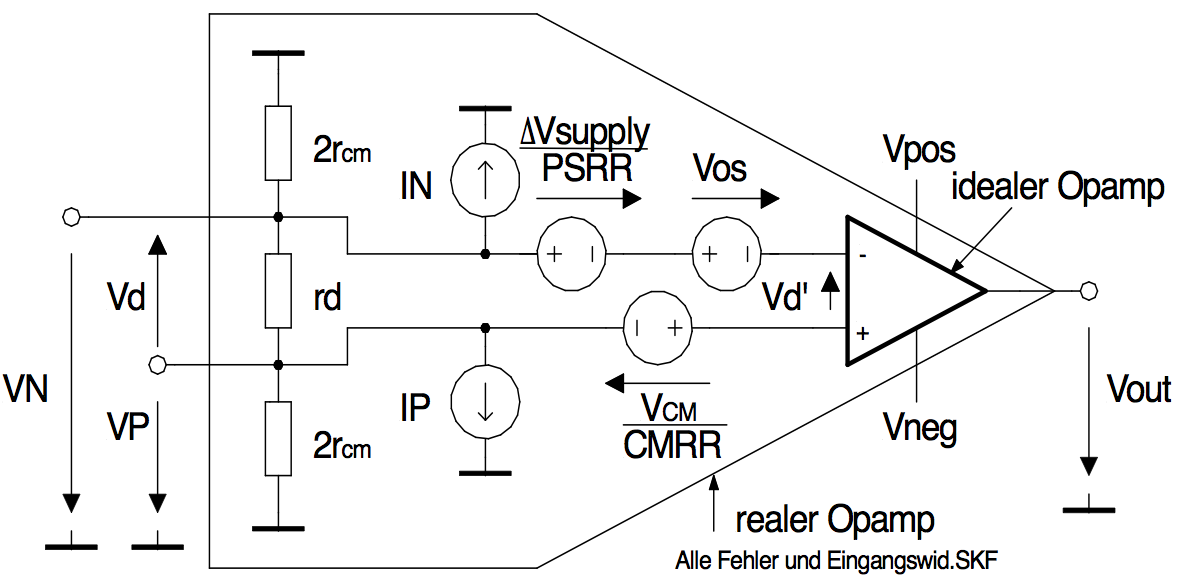
\includegraphics[width=6.5cm]{./bilder/OPAmpAlleFehler}
    \end{minipage}
\hrule
\hrule